% Options for packages loaded elsewhere
\PassOptionsToPackage{unicode}{hyperref}
\PassOptionsToPackage{hyphens}{url}
\PassOptionsToPackage{dvipsnames,svgnames,x11names}{xcolor}
%
\documentclass[
  authoryear,
  preprint,
  1p]{elsarticle}

\usepackage{amsmath,amssymb}
\usepackage{iftex}
\ifPDFTeX
  \usepackage[T1]{fontenc}
  \usepackage[utf8]{inputenc}
  \usepackage{textcomp} % provide euro and other symbols
\else % if luatex or xetex
  \usepackage{unicode-math}
  \defaultfontfeatures{Scale=MatchLowercase}
  \defaultfontfeatures[\rmfamily]{Ligatures=TeX,Scale=1}
\fi
\usepackage{lmodern}
\ifPDFTeX\else  
    % xetex/luatex font selection
\fi
% Use upquote if available, for straight quotes in verbatim environments
\IfFileExists{upquote.sty}{\usepackage{upquote}}{}
\IfFileExists{microtype.sty}{% use microtype if available
  \usepackage[]{microtype}
  \UseMicrotypeSet[protrusion]{basicmath} % disable protrusion for tt fonts
}{}
\makeatletter
\@ifundefined{KOMAClassName}{% if non-KOMA class
  \IfFileExists{parskip.sty}{%
    \usepackage{parskip}
  }{% else
    \setlength{\parindent}{0pt}
    \setlength{\parskip}{6pt plus 2pt minus 1pt}}
}{% if KOMA class
  \KOMAoptions{parskip=half}}
\makeatother
\usepackage{xcolor}
\setlength{\emergencystretch}{3em} % prevent overfull lines
\setcounter{secnumdepth}{5}
% Make \paragraph and \subparagraph free-standing
\makeatletter
\ifx\paragraph\undefined\else
  \let\oldparagraph\paragraph
  \renewcommand{\paragraph}{
    \@ifstar
      \xxxParagraphStar
      \xxxParagraphNoStar
  }
  \newcommand{\xxxParagraphStar}[1]{\oldparagraph*{#1}\mbox{}}
  \newcommand{\xxxParagraphNoStar}[1]{\oldparagraph{#1}\mbox{}}
\fi
\ifx\subparagraph\undefined\else
  \let\oldsubparagraph\subparagraph
  \renewcommand{\subparagraph}{
    \@ifstar
      \xxxSubParagraphStar
      \xxxSubParagraphNoStar
  }
  \newcommand{\xxxSubParagraphStar}[1]{\oldsubparagraph*{#1}\mbox{}}
  \newcommand{\xxxSubParagraphNoStar}[1]{\oldsubparagraph{#1}\mbox{}}
\fi
\makeatother


\providecommand{\tightlist}{%
  \setlength{\itemsep}{0pt}\setlength{\parskip}{0pt}}\usepackage{longtable,booktabs,array}
\usepackage{calc} % for calculating minipage widths
% Correct order of tables after \paragraph or \subparagraph
\usepackage{etoolbox}
\makeatletter
\patchcmd\longtable{\par}{\if@noskipsec\mbox{}\fi\par}{}{}
\makeatother
% Allow footnotes in longtable head/foot
\IfFileExists{footnotehyper.sty}{\usepackage{footnotehyper}}{\usepackage{footnote}}
\makesavenoteenv{longtable}
\usepackage{graphicx}
\makeatletter
\def\maxwidth{\ifdim\Gin@nat@width>\linewidth\linewidth\else\Gin@nat@width\fi}
\def\maxheight{\ifdim\Gin@nat@height>\textheight\textheight\else\Gin@nat@height\fi}
\makeatother
% Scale images if necessary, so that they will not overflow the page
% margins by default, and it is still possible to overwrite the defaults
% using explicit options in \includegraphics[width, height, ...]{}
\setkeys{Gin}{width=\maxwidth,height=\maxheight,keepaspectratio}
% Set default figure placement to htbp
\makeatletter
\def\fps@figure{htbp}
\makeatother

\makeatletter
\@ifpackageloaded{caption}{}{\usepackage{caption}}
\AtBeginDocument{%
\ifdefined\contentsname
  \renewcommand*\contentsname{Table of contents}
\else
  \newcommand\contentsname{Table of contents}
\fi
\ifdefined\listfigurename
  \renewcommand*\listfigurename{List of Figures}
\else
  \newcommand\listfigurename{List of Figures}
\fi
\ifdefined\listtablename
  \renewcommand*\listtablename{List of Tables}
\else
  \newcommand\listtablename{List of Tables}
\fi
\ifdefined\figurename
  \renewcommand*\figurename{Figure}
\else
  \newcommand\figurename{Figure}
\fi
\ifdefined\tablename
  \renewcommand*\tablename{Table}
\else
  \newcommand\tablename{Table}
\fi
}
\@ifpackageloaded{float}{}{\usepackage{float}}
\floatstyle{ruled}
\@ifundefined{c@chapter}{\newfloat{codelisting}{h}{lop}}{\newfloat{codelisting}{h}{lop}[chapter]}
\floatname{codelisting}{Listing}
\newcommand*\listoflistings{\listof{codelisting}{List of Listings}}
\makeatother
\makeatletter
\makeatother
\makeatletter
\@ifpackageloaded{caption}{}{\usepackage{caption}}
\@ifpackageloaded{subcaption}{}{\usepackage{subcaption}}
\makeatother
\journal{Psychometrika}

\ifLuaTeX
  \usepackage{selnolig}  % disable illegal ligatures
\fi
\usepackage[]{natbib}
\bibliographystyle{elsarticle-harv}
\usepackage{bookmark}

\IfFileExists{xurl.sty}{\usepackage{xurl}}{} % add URL line breaks if available
\urlstyle{same} % disable monospaced font for URLs
\hypersetup{
  pdftitle={Causes and effects in Dichotomous Comparative Judgments: an information-theoretical system with plausible mechanism},
  pdfauthor={Jose Manuel Rivera Espejo; Tine van van Daal; Sven De De Maeyer; Steven Gillis},
  pdfkeywords={comparative judgement, directed acycilc graph, causal
analysis, probabilistic statistics},
  colorlinks=true,
  linkcolor={blue},
  filecolor={Maroon},
  citecolor={Blue},
  urlcolor={Blue},
  pdfcreator={LaTeX via pandoc}}


\setlength{\parindent}{6pt}
\begin{document}

\begin{frontmatter}
\title{Causes and effects in Dichotomous Comparative Judgments: an
information-theoretical system with plausible mechanism}
\author[1]{Jose Manuel Rivera Espejo%
\corref{cor1}%
}
 \ead{JoseManuel.RiveraEspejo@uantwerpen.be} 
\author[1]{Tine van Daal%
%
}
 \ead{tine.vandaal@uantwerpen.be} 
\author[1]{Sven De Maeyer%
%
}
 \ead{sven.demaeyer@uantwerpen.be} 
\author[2]{Steven Gillis%
%
}
 \ead{steven.gillis@uantwerpen.be} 

\affiliation[1]{organization={University of Antwerp, Training and
education sciences},,postcodesep={}}
\affiliation[2]{organization={University of
Antwerp, Linguistics},,postcodesep={}}

\cortext[cor1]{Corresponding author}




        
\begin{abstract}
Dichotomous Comparative Judgment
\citep[DCJ,][@Pollitt\_2012b]{Pollitt_2012a} requires judges to evaluate
the relative manifestation of traits between pairs of stimuli, resulting
in a dichotomous outcome indicating which stimulus exhibits the trait
more strongly. Research has demonstrated DCJ's effectiveness and
reliability in various domains
\citep{Pollitt_2012b, Bartholomew_et_al_2018, vanDaal_et_al_2016, Lesterhuis_2018, Bartholomew_et_al_2020, Boonen_et_al_2020}.
Nevertheless, despite the method's widespread use, the literature lacks
a transparent depiction of the DCJ system and the plausible mechanisms
that generate the DCJ data. Particularly, there is no detailed
explanation of how different assessment factors can potentially
influence the observed DCJ data. This study aims to fill this gap by
applying the framework of causal analysis and Directed Acyclic Graphs
{[}DAG; \citet{Pearl_2009}{]}. Using this framework, the study will
construct a scientific model to elucidate the causal assumptions and
mechanisms inherent the system. This model will enable researchers to
draw inferences about causal relationships from DCJ data. Subsequently,
the study will translate this model into a probabilistic statistical
model, aiming to derive statistical estimands for different targets of
inference. The outcomes of this study will inform the planning of DCJ
experiments and hold significance for researchers or analysts involved
in education and assessment procedures who implement the DCJ
methodology.
\end{abstract}





\begin{keyword}
    comparative judgement \sep directed acycilc graph \sep causal
analysis \sep 
    probabilistic statistics
\end{keyword}
\end{frontmatter}
    

\section{Introduction}\label{sec-introduction}

In contemporary contexts, Thurstone's law of comparative judgment
\citeyearpar{Thurstone_1927} primarily refers to the method of
\emph{dichotomous} comparative judgment
\citep[DCJ,][]{Pollitt_2012a, Pollitt_2012b}. In DCJ, a judge assesses
the relative manifestation of a \emph{trait} within a pair of stimuli.
This assessment results in a dichotomous value indicating which stimulus
possesses a higher degree of the trait. After different judges perform
multiple rounds of pairwise comparisons, an outcome vector is produced.
This vector is modeled using the Bradley-Terry-Luce model
\citep[BTL,][]{Bradley_et_al_1952, Luce_1959}, which creates a score
that corresponds with the trait of interest. This score is then used to
rank the stimuli from lowest to highest or to evaluate the influence of
certain variables on the stimuli's positions in the ranking.

DCJ has proven effective in assessing competencies and traits
predominantly within the educational realm, as demonstrated by
\citet{Pollitt_2012b}, \citet{Jones_2015}, \citet{vanDaal_et_al_2016},
\citet{Bartholomew_et_al_2018}, \citet{Lesterhuis_2018},
\citet{Bartholomew_et_al_2020}, and \citet{Marshall_et_al_2020}.
However, its application transcends education, as exemplified by
\citet{Boonen_et_al_2020}. The methodology has also evolved to include
multiple, as opposed to pairwise comparisons
\citep{Luce_1959, Placket_1975}, and to accommodate comparisons with
ordinal outcomes \citep{Tutz_1986, Agresti_1992}. Overall, research
suggests that DCJ offers an alternative and efficient approach to
measurement and evaluation, characterized by its reliability and
validity \citep{Lesterhuis_2018, vanDaal_2020, Marshall_et_al_2020}.
Nevertheless, despite the method's widespread use, the literature does
not offer a clear representation of the plausible mechanisms that
generate DCJ data. Particularly, there is no depiction of the complexity
and the underlying assumptions of the DCJ system, nor how different
assessment factors can potentially influence the observed DCJ outcome.

According to \citet{Verhavert_et_al_2019} and \citet{vanDaal_2020},
several assessment factors interact and influence the method's outcome.
These factors include the number and characteristics of the stimuli,
their \emph{proximity} in terms of the assessed trait, the number of
comparison per stimulus, and the pairing algorithm used. Furthermore,
since the method relies on judges' assessments, the number and
characteristics of judges, their \emph{discrimination} abilities, and
the number of comparisons per judge also play pivotal roles. Moreover,
when the stimuli represent sub-units of higher-levels units, factors
such as the number and characteristics of these units, along with their
\emph{proximity} in terms of the assessed trait, can significantly
influence the outcome. For example, \citet{vanDaal_et_al_2016} assessed
the academic writing skills of university students (units) using
multiple argumentative essays (sub-units).

Although several studies have examined the individual impact of these
factors on the method's reliability
\citep{Bramley_2015, Pollitt_2012b, Bramley_et_al_2019, Verhavert_et_al_2019, Crompvoets_et_al_2022, vanDaal_et_al_2017, Gijsen_et_al_2021},
none, to the best of the authors' knowledge, have provided a transparent
depiction of the DCJ system and the mechanisms generating the DCJ
outcome. This study aims to fill this gap by representing DCJ within the
causal inference framework. Specifically, using the \emph{structural
approach} to causal inference
\citep{Wright_1921, Pearl_2009, Pearl_et_al_2016}, the study aims to
construct a scientific model. This model will elucidate the underlying
assumptions of the DCJ system, providing plausible mechanisms for how
the DCJ outcome is generated. Next, using a minimal set of assumptions,
the study will translate the scientific model into a probabilistic
statistical model. This model will produce statistical estimates to draw
inferences about plausible causal relationships within the DCJ system.

Ultimately, this research aims to extend the law of comparative judgment
initially proposed by \citet{Thurstone_1927} and provide a sound
probabilistic base for the statistical analysis of DCJ data.
Consequently, this research holds significance for researchers and
analysts involved in education and assessment procedures who implement
or design DCJ experiments.

\section{Preliminaries}\label{sec-prelim}

\subsection{The structural approach to causal
inference}\label{sec-prelim-structural}

In statistics, \emph{causal inference} refers to the process of
identifying the causes of a phenomenon and estimating their effects
using data \citep{Shaughnessy_et_al_2010, Neal_2020}. Unlike classical
statistical modeling, which focuses solely on summarizing data and
inferring associations, causal inference provides a coherent
mathematical representation for analyzing causes and counterfactuals
\citep{Pearl_2009}. Counterfactuals reflect scenarios \emph{contrary to
fact}, where alternative \emph{potential} outcomes have not been
observed and cannot be observed \citep{Neal_2020, Counterfactual_2024}.
Using counterfactuals, researchers can construct a theory of the world
that explains why specific causes have specific effects, and what
happens in the absence of those causes. Consequently, counterfactuals
represent the highest level of abstraction in causal inference
\citep{Pearl_et_al_2018}.

Several approaches to constructing counterfactuals and applying causal
inference exist, but two are particularly prominent: the potential
outcomes approach and the structural approach. The potential outcomes
approach, also known as the Neyman-Rubin causal model, was developed by
\citet{Neyman_et_al_1990} and \citet{Rubin_1974}. In contrast, the
structural approach was pioneered by \citet{Wright_1921}, and later
extended by Pearl \citep{Pearl_2009, Pearl_et_al_2016}. Both approaches
employ rigorous mathematical notation to characterize causal inference,
but they do so in different ways \citep{Neal_2020}. The potential
outcomes approach relies on counterfactual notation, whereas the
structural approach utilizes the do-operator and Structural Causal
Models \citep[SCM,][]{Pearl_2009, Pearl_et_al_2016}. Despite these
differences, both approaches provide methods for using experimental and
observational data to estimate causal effects \citep{Pearl_2010}.

However, the structural approach offers a significant advantage over the
potential outcomes approach by enabling the graphical representation of
systems through directed acyclic graphs
\citep[DAG,][]{Gross_et_al_2018, Neal_2020}. These graphical
representations provides a transparent depiction of a system's
complexity, revealing its underlying assumptions and the plausible
mechanisms generating the system's outcome. This capability aligns well
with the aims of this study. Consequently, the structural approach will
be the primary method used to address the study's research goal.

\begin{figure}

\centering{

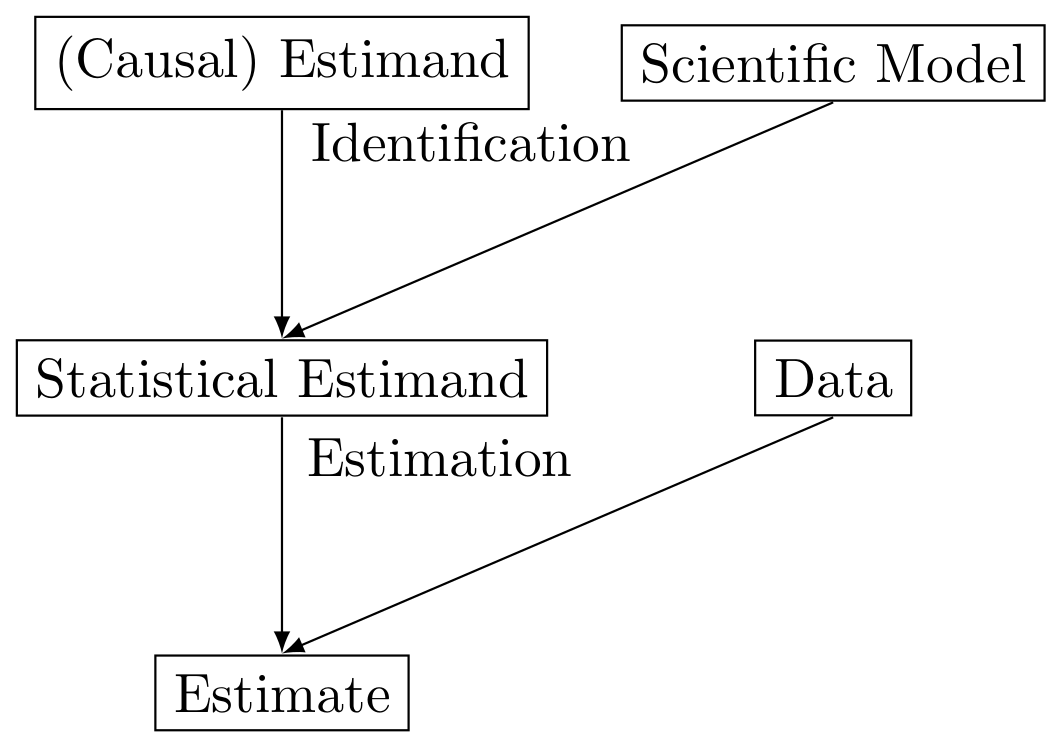
\includegraphics[width=0.4\textwidth,height=\textheight]{images/figures/IEflow.png}

}

\caption{\label{fig-IEflow}Identification-Estimation flowchart.
Extracted from \citet[32]{Neal_2020}}

\end{figure}%

\subsection{Graphs, DAGs and SCMs}\label{sec-prelim-graphs}

\subsection{The flow of association and
causation}\label{sec-prelim-flow}

\begin{figure}

\centering{

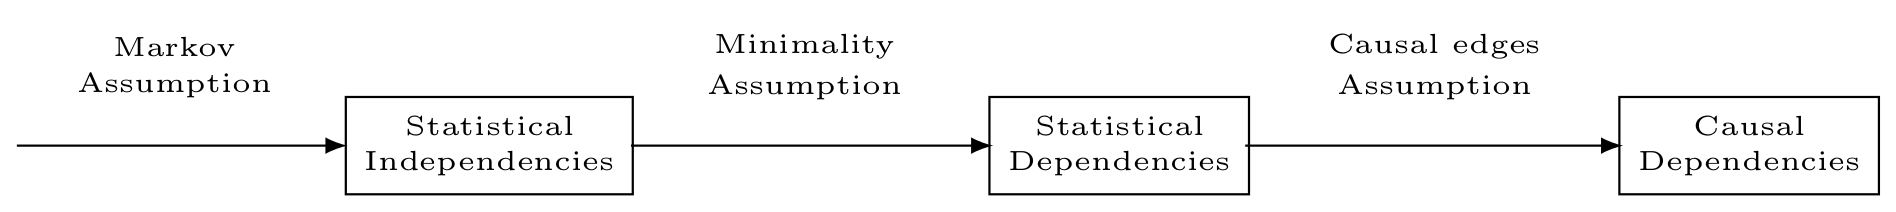
\includegraphics[width=1\textwidth,height=\textheight]{images/figures/ACflow.png}

}

\caption{\label{fig-ACflow}The flow of association and causation in
graphs. Extracted from \citet[31]{Neal_2020}}

\end{figure}%

\section{Theoretical framework}\label{sec-theory}

\subsection{A scientific model for the DCJ}\label{sec-theory-scientific}

\begin{figure}

\centering{

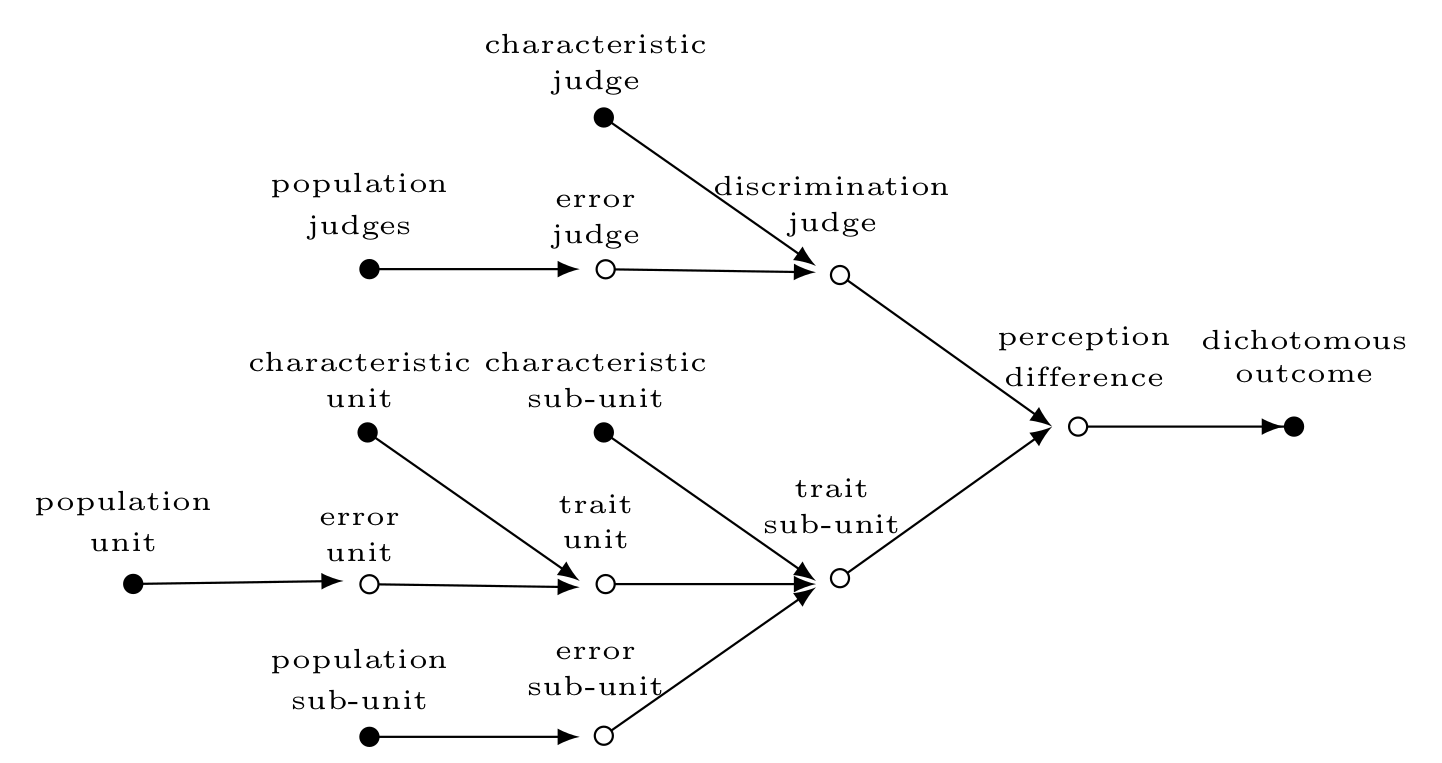
\includegraphics[width=0.8\textwidth,height=\textheight]{images/figures/SciModel_simp1.png}

}

\caption{\label{fig-SciModel_simp1}DCJ causal diagram, simplified
description}

\end{figure}%

\begin{figure}

\centering{

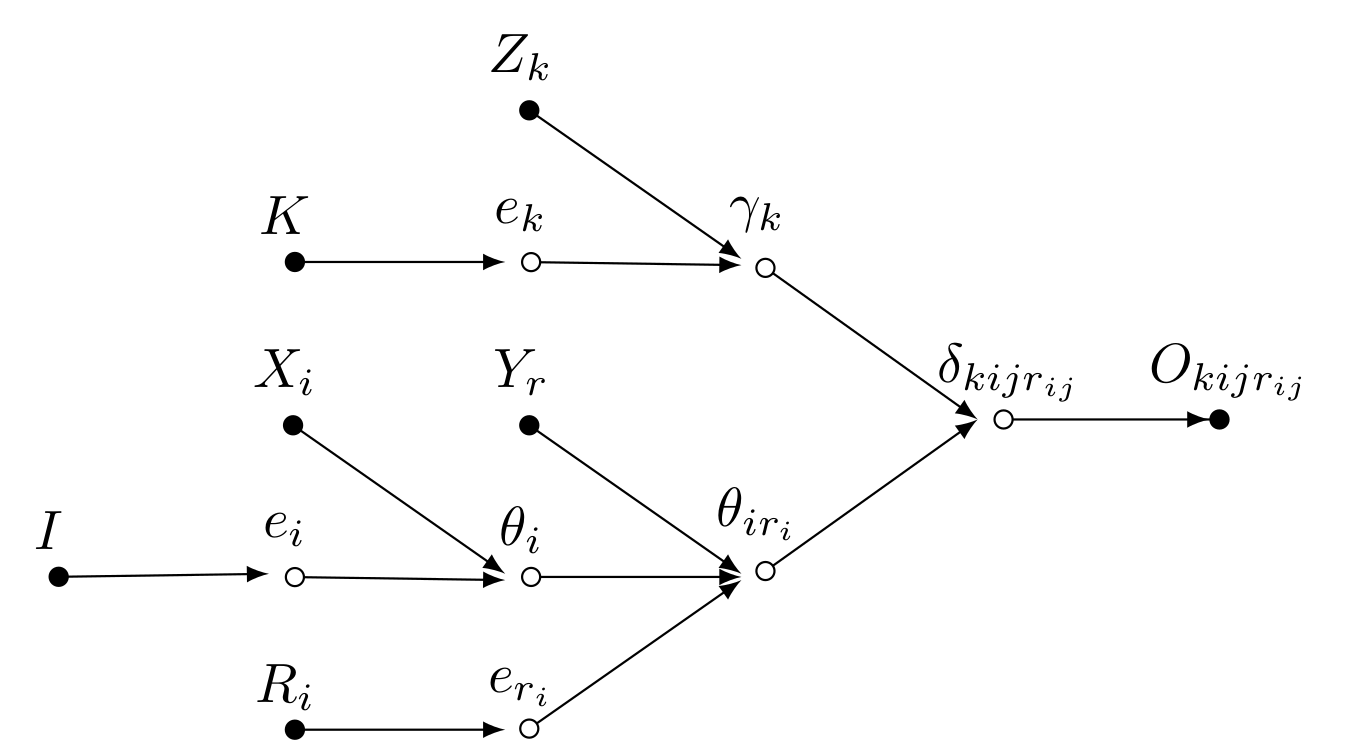
\includegraphics[width=0.7\textwidth,height=\textheight]{images/figures/SciModel_simp2.png}

}

\caption{\label{fig-SciModel_simp2}DCJ causal diagram, simplified
mathematical description}

\end{figure}%

\begin{figure}

\centering{

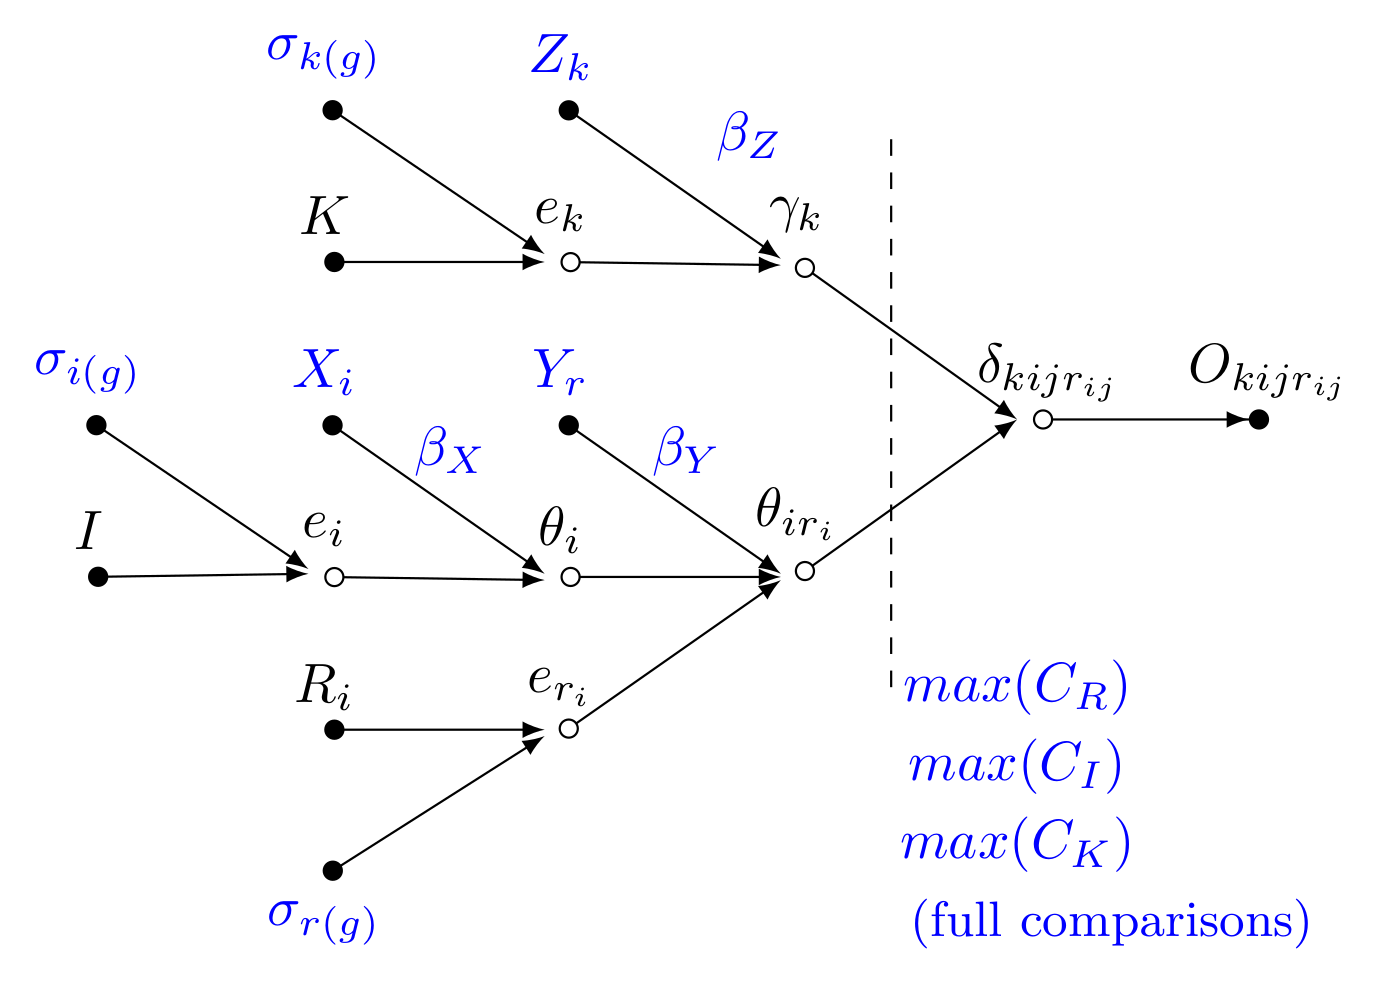
\includegraphics[width=0.7\textwidth,height=\textheight]{images/figures/SciModel_pop.png}

}

\caption{\label{fig-SciModel_pop}DCJ causal diagram, population
mathematical description}

\end{figure}%

\begin{figure}

\centering{

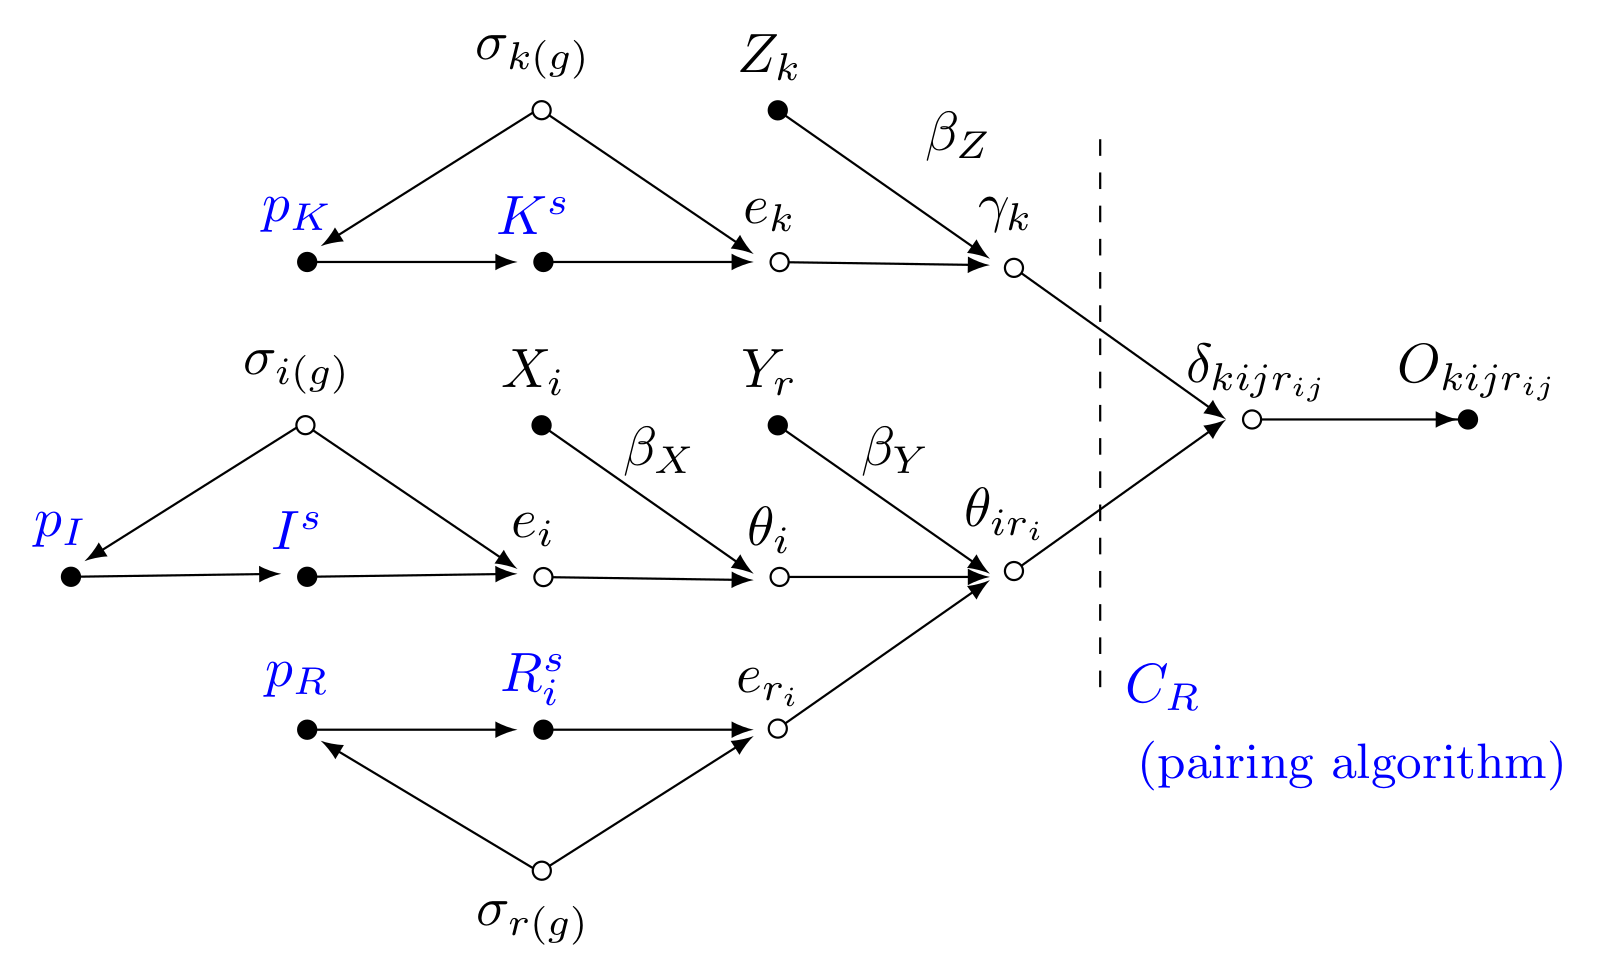
\includegraphics[width=0.8\textwidth,height=\textheight]{images/figures/SciModel_samp.png}

}

\caption{\label{fig-SciModel_samp}DCJ causal diagram, sample with
comparisons mathematical description}

\end{figure}%

\subsection{Probabilitics assumptions of the scientific
model}\label{sec-theory-probability}

\newcommand{\dsep}{\perp\!\!\!\perp}
\newcommand{\ndsep}{\not\!\perp\!\!\!\perp}

\begin{equation}\phantomsection\label{eq-StructuralModel}{
\begin{aligned}
  O_{kijr_{ij}} := & \; f_{O}( \delta_{kijr_{ij}} ) \\
  \delta_{kijr_{ij}} := & \; f_{D}( \gamma_{k}, \theta_{ir_{i}} ) \\
  \gamma_{k} := & \; f_{G}( Z_{k}, e_{k} ) \\
  \theta_{ir_{i}} := & \; f_{R}( \theta_{i}, Y_{r}, e_{r_{i}} ) \\
  \theta_{i} := & \; f_{T}( X_{i}, e_{i} ) \\
  & \; e_{k} \perp\!\!\!\perp e_{i} \\
  & \; e_{k} \perp\!\!\!\perp e_{r_{i}} \\
  & \; e_{i} \perp\!\!\!\perp e_{r_{i}}
\end{aligned}
}\end{equation}

\subsection{From the scientific to statistical
model}\label{sec-theory-statistics}

\begin{equation}\phantomsection\label{eq-StatModel_general}{
\begin{aligned}
  O_{kijr_{ij}} \sim & \; \text{Bernoulli}\left[ \; logit^{-1}\left( \delta_{kijr_{ij}} \right) \; \right] \\
  \delta_{kijr_{ij}} = & \; \gamma_{k}( \theta_{ir_{i}} - \theta_{jr_{j}} ) \\
  \gamma_{k} = & \; logit^{-1}\left[ \beta_{Z} Z_{k} + e_{k} \right] \\
  \theta_{ir_{i}} = & \; \theta_{i} + \beta_{Y} Y_{r} + e_{r_{i}}  \\
  \theta_{i} = & \; \beta_{X} X_{i} + e_{i}  \\
  e_{k} \sim & \; \text{Normal}(0, \sigma_{k(g)}) \\
  e_{i} \sim & \; \text{Normal}(0, \sigma_{i(g)}) \\
  e_{r_{i}} \sim & \; \text{Normal}(0, \sigma_{r(g)})
\end{aligned}
}\end{equation}

for identification purposes we can set
\(\frac{1}{G}\sum_{g=1}^{G} \sigma_{k(g)} = 0.02\),
\(\frac{1}{G}\sum_{g=1}^{G} \sigma_{i(g)} = 1\), and
\(\frac{1}{G}\sum_{g=1}^{G} \sigma_{r(g)} = 1\). A special case of this
would be to assume that the data comes from the same population, in that
case, \(\sigma_{k(g)} = \sigma_{k} = 0.02\),
\(\sigma_{i(g)} = \sigma_{i} = 1\)

\subsection{Let's talk about Thurstone}\label{sec-theory-thurstone}

Thurstone's comparative judgment \citet{Thurstone_1927} is based on the
formula: \[
X_{AB} = \frac{S_{A} - S_{B}}{\sigma_{AB}}
\]

where \(X_{AB}\) defines the comparative judgment outcome, \(S_{A}\) and
\(S_{B}\) are the modal discriminal processes,
\(\sigma_{AB} = \sqrt{ \sigma^{2}_{A} + \sigma^{2}_{B} + 2 \rho \sigma_{A} \sigma_{B}}\),
with \(\sigma_{A}\) and \(\sigma_{B}\) being the dispersion of
discriminal processes \(A\) and \(B\), respectively, and \(\rho\) the
correlation between discriminal processes.

The theory identifies five cases:

\begin{itemize}
\tightlist
\item
  \textbf{Case 1:} only constant \(\rho\) (not \(\rho_{ij}\))
\item
  \textbf{Case 2:} \(X_{ij}\) becomes \(X_{kij}\) with \(k=1, \dots, K\)
  judges (replication, not duplication)
\item
  \textbf{Case 3:} \(\rho = 0\), then
  \(\sigma_{AB} = \sqrt{ \sigma^{2}_{A} + \sigma^{2}_{B}}\)
\item
  \textbf{Case 4:} \(\sigma_{B}=\sigma_{A}+d\), then
  \(\lim_{d \leq 0.1\sigma_{A}} \sigma_{AB} = (\sigma_{A} + \sigma_{B}) /\sqrt{2}\)
\item
  \textbf{Case 5:} \(\sigma_{B}=\sigma_{A}\), then
  \(\sigma_{AB} = \sqrt{2}\sigma\)
\end{itemize}

Now using the DAG and statistical notation

\begin{equation}\phantomsection\label{eq-StatModel_thurstone}{
\begin{aligned}
  O_{kijr_{ij}} := & \; f_{O}( \delta_{kijr_{ij}} ) \\
  \delta_{kijr_{ij}} = & \; \gamma_{k}( \theta_{ir_{i}} - \theta_{jr_{j}} ) \\
  \gamma_{k} = & \; f_{G}( Z_{k}, e_{k} ) \\
  \theta_{ir_{i}} = & \; \theta_{i} + \beta_{Y} Y_{r} + e_{r_{i}}  \\
  \theta_{i} = & \; \beta_{X} X_{i} + e_{i}  \\
  e_{k} \sim & \; \text{Normal}(0, \sigma_{k(g)}) \\
  e_{i} \sim & \; \text{Normal}(0, \sigma_{i(g)}) \\
  e_{r_{i}} \sim & \; \text{Normal}(0, \sigma_{r(g)})
\end{aligned}
}\end{equation}

The theory identifies five cases:

\begin{itemize}
\tightlist
\item
  \textbf{Case 1:} only constant \(\rho \approx \sigma_{i}\)
\item
  \textbf{Case 2:} now judges are separated by using \(\gamma_{k}\)
\item
  \textbf{Case 3:} \(\rho \approx \sigma_{e_{i}} = 0\) (no nesting of
  texts on students), then
  \(\sigma_{AB} = \sqrt{ \sigma^{2}_{A} + \sigma^{2}_{B}}\)
\item
  \textbf{Case 4:} \(\sigma_{B}=\sigma_{A}+d\), then
  \(\lim_{d \leq 0.1\sigma_{A}} \sigma_{AB} = (\sigma_{A} + \sigma_{B}) /\sqrt{2}\)
\item
  \textbf{Case 5:} \(\sigma_{B}=\sigma_{A}\), then
  \(\sigma_{AB} = \sqrt{2}\sigma\)
\end{itemize}

But now can we see other scenarios than just those 5 cases?

\begin{itemize}
\tightlist
\item
  consider different \(\rho \approx \sum_{p=1}^{P} \sigma_{p}\),
  depending on \(P\) nesting structures
\item
  we can now investigate \(\gamma_{k}\)
\item
  we can assume \(\sigma_{B} \neq \sigma_{A}\), no need for results on
  the limit
\end{itemize}

\section{Discussion}\label{sec-discuss}

\subsection{Findings}\label{sec-discuss-finding}

\subsection{Limitations and further
research}\label{sec-discuss-limitations}

\section{Conclusion}\label{sec-conclusion}

\newpage{}

\section*{Declarations}\label{declarations}
\addcontentsline{toc}{section}{Declarations}

\textbf{Funding:} The project was founded through the Research Fund of
the University of Antwerp (BOF).

\textbf{Conflict of interests:} The authors declare no conflict of
interest.

\textbf{Ethics approval:} The University of Antwerp Research Ethics
Committee has confirmed that no ethical approval is required.

\textbf{Consent to participate:} Not applicable

\textbf{Consent for publication:} All authors have read and agreed to
the published version of the manuscript.

\textbf{Availability of data and materials:} No data was utilized in
this study

\textbf{Code availability:} All the code utilized in this research is
available in the digital document located at:
\url{https://jriveraespejo.github.io/paper2_manuscript/}.

\textbf{Authors' contributions:} \emph{Conceptualization:} S.G., S.DM.,
T.vD., and J.M.R.E; \emph{Methodology:} S.DM., T.vD., and J.M.R.E;
\emph{Software:} J.M.R.E.; \emph{Validation:} J.M.R.E.; \emph{Formal
Analysis:} J.M.R.E.; \emph{Investigation:} J.M.R.E; \emph{Resources:}
S.G., S.DM., and T.vD.; \emph{Data curation:} J.M.R.E.; \emph{Writing -
original draft:} J.M.R.E.; \emph{Writing - review \& editing:} S.G.,
S.DM., and T.vD.; \emph{Visualization:} J.M.R.E.; \emph{Supervision:}
S.G. and S.DM.; \emph{Project administration:} S.G. and S.DM.;
\emph{Funding acquisition:} S.G. and S.DM.

\newpage{}

\section{Appendix}\label{sec-appendix}

\subsection{Additional definitions}\label{sec-appA}

\textbf{Counterfactual:}

\subsection{Why do we need to estimate judges'
abilities?}\label{sec-appB}

\newpage{}

\subsection*{References}\label{references}
\addcontentsline{toc}{subsection}{References}

\renewcommand{\bibsection}{}
\bibliography{references.bib}





\end{document}
